\section{יחידה 8: ייצוגים גרפיים, התפלגות וצפיפות}

יחידה זו עוסקת באופן שבו מתארים משתנים כמותיים באמצעות גרפים,
ובמעבר ההדרגתי מייצוג של נתונים במדגם
לייצוג תאורטי של משתנה באוכלוסייה.

המעבר מתבצע בשלבים:
\begin{itemize}
\item ייצוג נתונים במדגם (שכיחויות)
\item ייצוג רציף באמצעות היסטוגרמה
\item מעבר לצפיפות ולשטחים
\item פונקציית צפיפות כמודל אוכלוסייה
\end{itemize}

---

\subsection{מהי התפלגות}

התפלגות מתארת כיצד ערכי המשתנה \textbf{מתפזרים} על פני תחום הערכים האפשריים.
לא מדובר בערך יחיד, אלא בתיאור של מבנה הנתונים כולו:
איפה יש ריכוז, איפה יש דלילות, ומה צורת הפיזור.

---

\subsection{ייצוג נתונים במדגם}

כאשר עובדים עם מדגם סופי, הנתונים ניתנים לספירה.
בשלב זה אנו מתארים את הנתונים באמצעות \textbf{שכיחויות}.

\subsubsection{דיאגרמת מקלות}

דיאגרמת מקלות מתאימה למשתנים בדידים או קטגוריאליים.

מאפיינים:
\begin{itemize}
\item ציר $X$ – קטגוריות
\item ציר $Y$ – שכיחות או שכיחות יחסית
\item אין משמעות למרחקים בין הקטגוריות
\end{itemize}

גובה המקל מייצג ישירות את מספר התצפיות בקטגוריה.

---

\subsection{מעבר למשתנים רציפים}

כאשר המשתנה כמותי ורציף (למשל: זמן, גובה, משקל),
לא ניתן לייצג כל ערך בנפרד.
במקום זאת מחלקים את התחום לקטגוריות רציפות (bins).

---

\subsection{היסטוגרמה}

היסטוגרמה היא ייצוג גרפי של משתנה רציף במדגם.

מאפיינים:
\begin{itemize}
\item ציר $X$ – תחומים רציפים
\item העמודות צמודות
\item לכל עמודה יש רוחב וגובה
\end{itemize}

---

\subsection{למה גובה העמודה הוא צפיפות ולא שכיחות}

נניח קטגוריה ברוחב $w_i$ עם שכיחות $f_i$.

אם היינו מציבים את גובה העמודה כשכיחות,
אז השטח היה:
\[
\text{שטח} = f_i \cdot w_i
\]
ומחלקות רחבות היו מקבלות שטח גדול יותר גם בלי יותר נתונים.

לכן מגדירים:

\[
\text{צפיפות} = \frac{f_i}{w_i}
\]

ואז מתקיים:
\[
\text{שטח} = \text{צפיפות} \times \text{רוחב} = f_i
\]

\textbf{מסקנה:}  
השטח מייצג שכיחות – לא הגובה.

---

\subsection{צפיפות יחסית ונירמול}

כדי לעבור משכיחות להסתברות מדגמית,
מחלקים את השכיחות ב־$n$.

\[
\text{צפיפות יחסית} = \frac{f_i}{n \cdot w_i}
\]

ואז:
\[
\text{שטח העמודה} = \frac{f_i}{n}
\]

כלומר: השטח מייצג \textbf{הסתברות מדגמית},
וסכום כל השטחים שווה ל־1.

---

\subsection{מעבר מהיסטוגרמה לפונקציית צפיפות}

כאשר:
\begin{itemize}
\item גודל המדגם גדל
\item רוחב הקטגוריות קטן
\end{itemize}

ההיסטוגרמה מתקרבת לעקומה רציפה.

בגבול מתקבלת \textbf{פונקציית צפיפות} $f(x)$.

---

\subsection{פונקציית צפיפות}

\begin{english}
A probability density function $f(x)$ satisfies:
\[
f(x) \ge 0
\qquad\text{and}\qquad
\int_{-\infty}^{\infty} f(x)\,dx = 1
\]
\end{english}

ההסתברות לקבל ערך בתחום $[a,b]$ היא:
\begin{english}
\[
P(a \le X \le b) = \int_a^b f(x)\,dx
\]
\end{english}

---

\subsection{למה ההסתברות לערך מדויק היא אפס}

עבור משתנה רציף:
\begin{english}
\[
P(X = x) = \int_x^x f(t)\,dt = 0
\]
\end{english}

נקודה היא קטע באורך אפס, ולכן השטח שלה אפס.

זה \textbf{לא} אומר שהערך בלתי אפשרי,
אלא שאין לו משקל הסתברותי.

---

\subsection{צורות התפלגות}

\subsubsection{התפלגות סימטרית}
\begin{itemize}
\item ממוצע = חציון = שכיח
\end{itemize}

\subsubsection{הטיה ימנית (זנב ימני)}
\[
\text{שכיח} < \text{חציון} < \text{ממוצע}
\]

\subsubsection{הטיה שמאלית (זנב שמאלי)}
\[
\text{ממוצע} < \text{חציון} < \text{שכיח}
\]

---

\subsection{ההתפלגות הפעמונית}

התפלגות נורמלית היא סימטרית ובעלת צורת פעמון,
ומאופיינת על ידי:
\begin{itemize}
\item $\mu$ – תוחלת
\item $\sigma$ – סטיית תקן
\end{itemize}

סטיית התקן קובעת את רוחב ההתפלגות:
סטיית תקן גדולה → פיזור רחב יותר.

---

\subsection{פוליגון}

פוליגון מתקבל מחיבור נקודות האמצע של מחלקות ההיסטוגרמה,
כאשר ציר $Y$ מייצג צפיפות.

גם כאן:
\textbf{השטח שמתחת לפוליגון מייצג שכיחות או הסתברות}.

---

\subsection{דגש מסכם ליחידה}

העיקרון המאחד של היחידה:
\[
\textbf{במשתנים רציפים — הסתברות מיוצגת על ידי שטח}
\]

המעבר:
\[
\text{מדגם} \rightarrow
\text{היסטוגרמה} \rightarrow
\text{צפיפות} \rightarrow
\text{פונקציית צפיפות}
\]

\subsection{המעבר מהיסטוגרמה לעקומת צפיפות}
ככל שנגדיל את המדגם ונצמצם את רוחב המחלקות, ההיסטוגרמה תהפוך לעקומה רציפה. השטח מתחת לעקומה תמיד יהיה שווה ל-1.

\begin{figure}[H]
\centering
\begin{english}
\begin{tikzpicture}[xscale=1.2, yscale=3]
  % עמודות היסטוגרמה
  \foreach \x/\h in {-2/0.1, -1.5/0.3, -1/0.6, -0.5/0.9, 0/1, 0.5/0.9, 1/0.6, 1.5/0.3, 2/0.1}
    \draw[fill=blue!10] (\x,0) rectangle (\x+0.5,\h);
  
  % עקומת צפיפות
  \draw[thick, red, smooth, domain=-2.5:3] plot (\x, {exp(-(\x-0.25)^2/1.2)});
  
  \draw[->] (-3,0) -- (3.5,0) node[right] {$X$};
  \node[red] at (1.5,0.8) {צפיפות $f(x)$};
\end{tikzpicture}
\end{english}
\caption{היסטוגרמה של המדגם מול פונקציית צפיפות של האוכלוסייה.}
\end{figure}

\begin{figure}[H]
\centering
\begin{english}
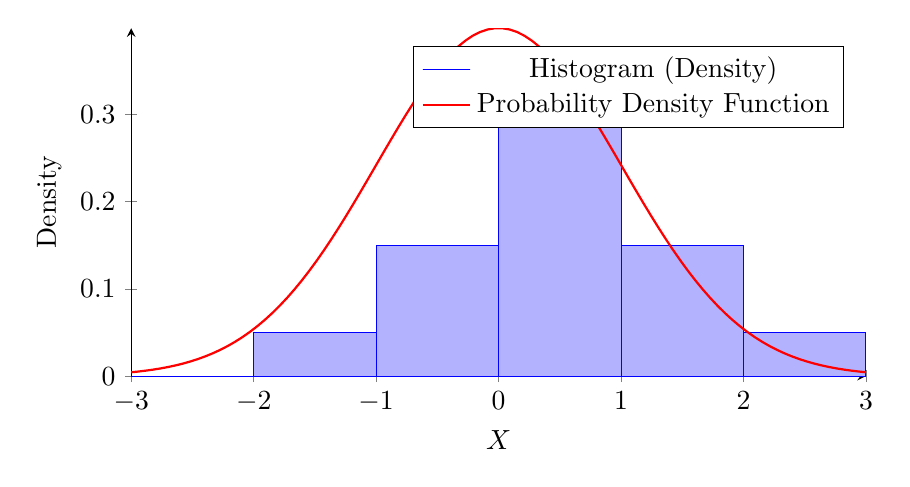
\begin{tikzpicture}
\begin{axis}[
    width=0.9\textwidth,
    height=6cm,
    xlabel={$X$},
    ylabel={Density},
    ymin=0,
    domain=-3:3,
    samples=100,
    axis lines=left,
    legend style={at={(0.97,0.95)},anchor=north east}
]

% היסטוגרמה (קירוב באמצעות עמודות)
\addplot[ybar interval, fill=blue!30, draw=blue]
coordinates {
(-3,0) (-2,0.05) (-1,0.15) (0,0.3) (1,0.15) (2,0.05) (3,0)
};

% עקומת צפיפות נורמלית
\addplot[thick, red]
{1/sqrt(2*pi)*exp(-x^2/2)};

\legend{Histogram (Density), Probability Density Function}

\end{axis}
\end{tikzpicture}
\end{english}
\caption{המעבר מהיסטוגרמה למדד צפיפות רציף. השטח מייצג הסתברות.}
\end{figure}

\begin{figure}[H]
\centering
\begin{english}
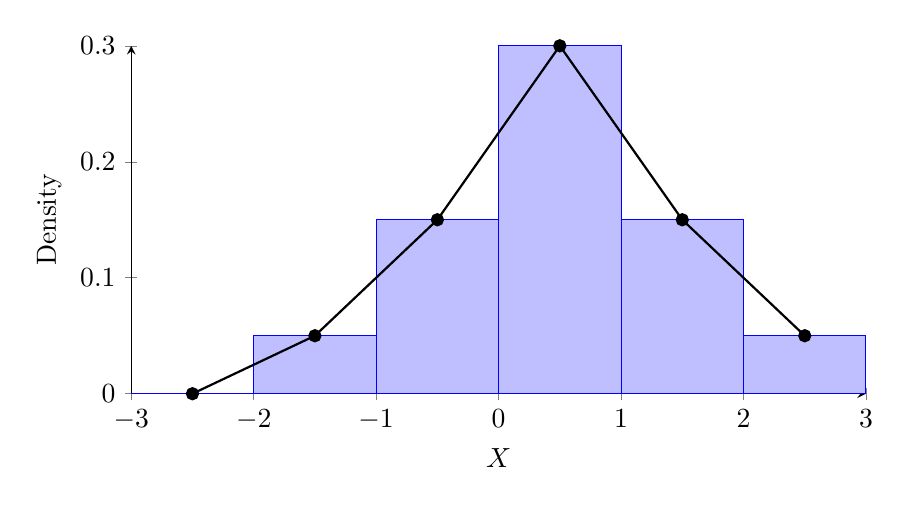
\begin{tikzpicture}
\begin{axis}[
    width=0.9\textwidth,
    height=6cm,
    xlabel={$X$},
    ylabel={Density},
    ymin=0,
    axis lines=left
]

% Histogram (density) — intervals: [x_i, x_{i+1})
\addplot[ybar interval, fill=blue!25, draw=blue]
coordinates {
(-3,0) (-2,0.05) (-1,0.15) (0,0.30) (1,0.15) (2,0.05) (3,0)
};

% Density polygon — midpoints of the same intervals
\addplot[thick, mark=*]
coordinates {
(-2.5,0)
(-1.5,0.05)
(-0.5,0.15)
(0.5,0.30)
(1.5,0.15)
(2.5,0.05)
};

\end{axis}
\end{tikzpicture}
\end{english}
\caption{היסטוגרמה (צפיפות) ופוליגון צפיפות: הקו מחבר את מרכזי המחלקות בגובה העמודות.}
\end{figure}
